\documentclass{beamer}
\usetheme{Copenhagen}
\usepackage{polyglossia}
\usepackage{tabu}
\usepackage{multicol}
\setdefaultlanguage{english}

\title{So you're a Linux kernel developer? \\Name all subsytems.}
%\subtitle{Name all subsystems.}

%\usetheme{lucid}
\begin{document}
	\frame {
		\titlepage
		\includegraphics[scale=0.25]{OTH_LOGO.png}
	}

	%\begin{frame}
	%\frametitle{Topics}
	%	\begin{block}{}

	%	\end{block}
	%\end{frame}

	% TODO: TIKZ-Diagramm um Section Graph zu verdeutlichen
	%TODO: Coole Trivia zu neuen Subsystemen einholen, damit man mehr darüber reden kann
	% TODO: alles neu plotten
	%TODO: integrieren
	%TODO; überdenken: vllt mehr auf PaStA eingehen? Live-Demo? Das Labor mehr vorstellen? 
	%TODO: Fragestellungen, die man beantworten möchte/Probleme, die man lösen möchte
	%TODO: alle Kontributoren, Collaboration mit der Uni Passau, dass alles, was wir machen, auch Anwendung hat und der Community was bringen soll, Elisa erwähnen
	%tODO: nochmal am Ende sagen, wer wir alle sind


	\begin{frame}
	\frametitle{Speaker Introduction}
	\begin{columns}
		\begin{column}{0.55\textwidth}
			\begin{block}{Pia Eichinger}
			\begin{itemize}
			\item Student at the University of Applied Sciences in Regensburg
			%\item Currently in a Masters of Applied Research Programme, researching database-specific kernels
			\item Researched organisational and maintenance structure of the Linux kernel
			\end{itemize}
			\end{block}
		\end{column}
		\begin{column}{0.4\textwidth}
     		\includegraphics[width=1.0\textwidth]{pics/speaker_piaei.jpg}
		\end{column}
	\end{columns}
	\end{frame}

	\begin{frame}
	\frametitle{Bachelor Thesis - Motivation and Beginnings}
		\begin{block}{Linux + Safety Critical Environments}
			= Development Process: Major certification challenges
		\end{block}
		\Rightarrow Ex post facto analysis\\ %TODO: Ex post facto analysis\\
		\Rightarrow Process characterisation with hindsight

		\begin{alertblock}{Goal}
			Use analytical tools for quantitive software engineering to analyse patch integration in the Linux kernel repository. %TODO: Aufspalten Mit analytischem quantitativen Softwareengineering wird des gmacht
		\end{alertblock}
	\end{frame}



	\begin{frame}
	\frametitle{Bachelor Thesis - Motivation and Beginnings}
		\begin{block}{Patch Integration - Maintainers Hierarchy Traversal}
			Developer $\Rightarrow$ Maintainer $\Rightarrow$ Subsystem Maintainer $\Rightarrow$ Mainline
		\end{block}
		\begin{block}{Original Research Questions}
			\begin{itemize}
				\item Was a patch conformingly integrated? (Integrated by a relevant maintainer according to MAINTAINERS)
				\item Did the patch traverse the maintainers hierarchy?
				%\item How do the different subsystems compare in regards to integration?
			\end{itemize}
		\end{block}
	\end{frame}


	\begin{frame}
	\frametitle{The Subsystem Problem}
		\begin{alertblock}{Only problem is ...}
			\begin{itemize}
				\item \textbf{... where can I find the maintainers hierarchy?}
				\item \textbf{... where can I find the documentation on all subsystems?}
				\item \textbf{... what exactly \textit{is} a subsystem even?}
			\end{itemize}
		\end{alertblock}
	\end{frame}


	\begin{frame}
	\frametitle{The Subsystem Problem - What is a subsystem?}
	%\begin{block}{Documentation: Early-stage Planning in the Linux Kernel Development Process}
	%	"Again, the MAINTAINERS file is	the place to start.  That file tends to not always be up to date, though, and not all \textbf{subsystems} are represented there."

	%	$\Rightarrow$ Every single entry in MAINTAINERS is one subsystem.
	%\end{block}

	%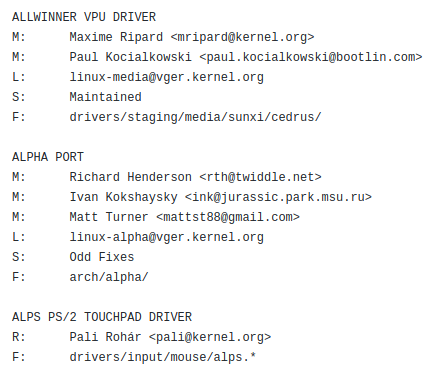
\includegraphics[scale=0.25]{pics/MAINTAINERSbild.png}
	\begin{columns}
		\begin{column}{0.55\textwidth}
			\begin{block}{Docs: Early-stage Planning}
			"Again, the MAINTAINERS file is	the place to start.  That file tends to not always be up to date, though, and not all \textbf{subsystems} are represented there."
			\end{block}
     		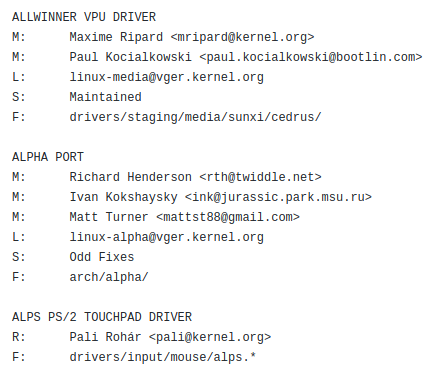
\includegraphics[width=0.6\textwidth]{pics/MAINTAINERSbild.png}
		\end{column}
		\begin{column}{0.4\textwidth}
		$\Rightarrow$ Every single entry in MAINTAINERS is one subsystem.
		\end{column}
	\end{columns}
	\end{frame}


	\begin{frame}
	\frametitle{The Subsystem Problem - What is a subsystem?}
     	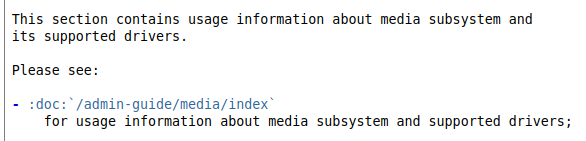
\includegraphics[width=0.6\textwidth]{pics/Media_subsystem.png}

	\begin{block}{But... }
		\begin{itemize}
		\item Not a single "Media" or "Media Subsystem" entry in MAINTAINERS
		\item Over 100 "subsystems" \textit{containing} the word "Media"
		\end{itemize}
	\end{block}
	$\Rightarrow$ So which one is it? All of them together? Some of them together? Any single \textit{one} of them?
	\end{frame}

	\begin{frame} %TODO: Entries in MAINTAINERS: sections, rechts in Bsp veranschaulichen
	\frametitle{Subsystem Definition}
		\begin{block}{Definition: Subsystem}
			We call the entries in MAINTAINERS \textbf{sections}.

			Two sections are \textbf{thematically related}, if they share a lot files measured in Lines of Code (LoC).

			A subsystem is a grouping of \textbf{strongly thematically related} sections.
		\end{block}
	\end{frame}

	\begin{frame}
	\frametitle{Bachelor Thesis - Change of Research Question}
		\begin{block}{No clear listing of subsystems}
			$\Rightarrow$ Let's find out!
		\end{block}

		\begin{block}{New Research Questions}
			\begin{itemize}
				\item Was a patch conformingly integrated? (Integrated by a relevant maintainer according to MAINTAINERS)
				\item Which most influential subsystems can we detect through clustering and grouping sections based on thematical relations?
			\end{itemize}
		\end{block}
	\end{frame}


	\begin{frame}
	\frametitle{Definition: Section Graph}
		\begin{alertblock}{Definition: Section Graph}
			\begin{itemize}
				\item Undirected Graph
				\item \textit{Vertices}: Every single section of maintainers becomes one vertex
				\item \textit{Vertex Weight}: accumulated LoC of all relevant files for the section
				\item \textit{Edge}: Do two sections share LoC? Yes $\Rightarrow$ Edge
				\item \textit{Edge Weight}: accumulated LoC of all shared files of both sections
			\end{itemize}
		\end{alertblock}

		$\Rightarrow$ Find subsystems by finding clusters with common community detection algorithms (Walktrap) %TODO: etablierte Verfahren, referenziere Paper Mitchell Choblins Mauerer, Abels, wir ham Gedanken drüber gmacht, etabliertes Verfahren, wurde damit entwickelt und wir nehmen ned IRGENDWAS
	\end{frame}

	\begin{frame}
	\frametitle{Top-20\% Section Graph}
	\begin{center}
	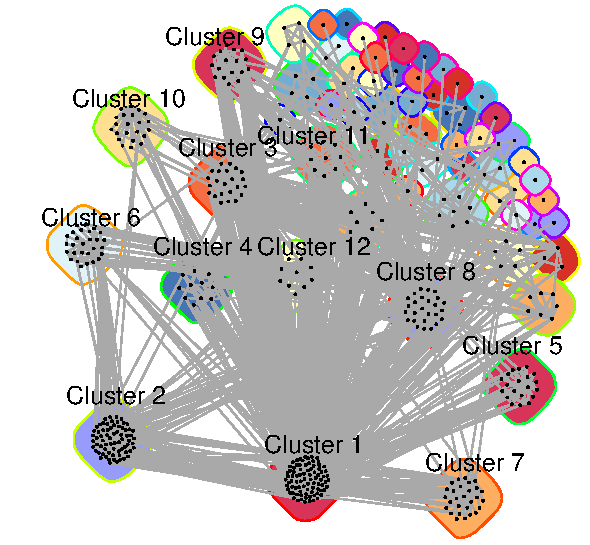
\includegraphics[scale=0.6]{pics/final_graph_with_texts_cropped.pdf}
	\end{center}
	\end{frame}



	\begin{frame}
	\frametitle{Cluster Discussion and Terminology}
		\begin{alertblock}{Cluster Discussion}
			\begin{itemize}
				\item Analyse and discuss each major cluster as \textbf{isolated graph}
				\item "Recluster" the isolated cluster graph again from within using walktrap
			\end{itemize}
		\end{alertblock}
		
		\begin{block}{Terminology}
			\begin{itemize}
				\item Isolated cluster as own graph: \textbf{Cluster Graph}
				\item Cluster found within cluster graph: \textbf{Subcluster}
				\item Vertex degree within entire section graph: \textbf{Outer Degree}
				\item Vertex degree within cluster graph: \textbf{Inner Degree}
			\end{itemize}
		\end{block}
	\end{frame}



	\begin{frame}
	\frametitle{Reminder: Research Questions}
		\begin{alertblock}{Integration Research Question}
		Was a patch conformingly integrated? (Integrated by a relevant maintainer according to MAINTAINERS)
		\end{alertblock}

		\begin{block}{TL;DR}
			\begin{itemize}
				\item Research recent patches in mainline and by which maintainer they were originally committed
				\item Maintainer relevant according to get\_maintainer.pl? $\Rightarrow$ "correctly" integrated
				\item Research on all major lists with highest patch traffic
				\item Go into detail as to \textit{why} a maintainer might have "incorrectly" committed patches outside of their relevant subsystem
			\end{itemize}
		\end{block}
	\end{frame}



	\begin{frame}
	\frametitle{Possible Reasons for "false" Integrations}
	\begin{block}{Two Examples of "wrong" Committers für intel-gfx}
		\begin{itemize}
			\item Daniel Vetter, Maintainer for DRM DRIVERS und DRM DRIVER FOR VIRTUAL KERNEL MODESETTING (VKMS)
			\item Maarten Lankhorst, Maintainer for DRM DRIVERS AND MISC GPU PATCHES
		\end{itemize}
	\end{block}
	\begin{block}{All relevant sections for the mailing list intel-gfx}
		\begin{itemize}
			\item INTEL DRM DRIVERS (excluding Poulsbo, Moorestown and derivative chipsets)
			\item INTEL GVT-g DRIVERS (Intel GPU Virtualization) $\Rightarrow$ relevant files in drivers/gpu/drm/i915/gvt/ %TODO: hervorheben, dass wir die Personen nicht hervorheben wollen, sondern nur analysieren, was denn so gemacht wird und quantifizieren. Namen rausnehmen. Weder finger pointing, es geht uns nur drum, Klassifikationen zu machen
			%TODO: Future work
		\end{itemize}
	\end{block}
	\end{frame}


\end{document}
